%%%%%%%%%%%%%%%%%%%%%%%%%%%%%%%%%%%%%%%%%%%%%%%%%%%%%%%%%%%%%%%%%%%%%%%%%%%%%%%%%%%%%
% Template revision history:
% BS02022: Revised by Sukumar Natarajan, s.natarajan@bath.ac.uk
% BS2021: Revised by Filip Jorissen, filip.jorissen@kuleuven.be
% BS2019: Revised by Alessandro Prada, alessandro.prada@unitn.it
% BS2017: Initial version by Michael Wetter, mwetter@lbl.gov
%%%%%%%%%%%%%%%%%%%%%%%%%%%%%%%%%%%%%%%%%%%%%%%%%%%%%%%%%%%%%%%%%%%%%%%%%%%%%%%%%%%%%

\documentclass[twocolumn, a4paper,10pt]{article}
\usepackage[top=2.5cm, bottom=2.5cm, left=2.0cm, right=2.0cm,
columnsep=0.8cm]{geometry}
\usepackage{enumitem}
\usepackage[hyphens]{url}
\usepackage[colorlinks,allcolors=blue]{hyperref}
\usepackage{boxedminipage}
\usepackage{nopageno}
\usepackage{graphicx}
\usepackage{amsmath}
\usepackage{natbib}
\usepackage[font=it]{caption}
\usepackage[usenames,dvipsnames]{xcolor}
\usepackage{listings}
\usepackage{caption}
\usepackage{subcaption}
\usepackage{bookmark}
\usepackage{float}
\DeclareCaptionType[within=section]{mat}[Matrix]


%-----------------------------SET SKIP SPACES -------------------------------------------------------------------
\setlength{\abovecaptionskip}{0pt}
\setlength{\belowcaptionskip}{3pt}
\setlength{\parindent}{0pt}
\setlength{\parskip}{3pt}
%\renewcommand{\baselinestretch}{0.7}
% FOR enumerates
\setlist{itemsep=-0.1cm,topsep=0.1cm,labelsep=0.3cm}
\setenumerate{leftmargin=*}
\setcounter{secnumdepth}{-1}
%-----------------------------SET FONTS -------------------------------------------------------------------
% Set fonts for title, section and subsection headings
\makeatletter
\renewcommand\title[1]{\gdef\@title{\fontsize{12pt}{2pt}\bfseries{#1}}}
\makeatletter
\renewcommand\section{\@startsection{section}{1}{\z@}{3pt}{3pt}{\normalfont\large\bfseries}}
% \normalfont\large
\makeatletter
\renewcommand\subsection{\@startsection{subsection}{1}{\z@}{\z@}{\z@}{\normalfont\normalsize\bfseries}}
\makeatletter
\renewcommand\subsection{\@startsection{subsection}{1}{\z@}{\z@}{0.1pt}{\normalfont\normalsize\bfseries}}
\renewcommand\refname{References}
%END OF THE SETUP
%%%%%%%%%%%%%%%%%%%%%%%%%%%%%%%%%%%%%%%%%%%%%%%%%%%%%%%%%%%%

%%%%%%%%%%%%%%%%%%%%%%%%   TITLE   %%%%%%%%%%%%%%%%%%%%%%%%%%%%%%%
%%% Please keep the \vspace{4pt} at the top
\title{%
Project Report for: Neapolitan Card Classifier\\																								% Line 1
%%% Please keep the \vspace{4pt} between lines in the title
\vspace{4pt}
Real world cases and Humanitarian implications \[LM-32 a.a. 2023/2024\]
} 																																% Line 2 
%If there is no second line then just put \phantom{Line 2} here
%%% Change or delete text before "\\" on the lines below to keep the layout but don't remove the "\\"
%%% Do not exceed more than 6 lines for authors and affiliations
\author{																																														% Line 3
Emmanuele Virginio Coppola$^1$\\ 																										% Line 4
$^1$ emmanuele.coppola@studenti.unitn.it\\ 																																	% Line 5
% comment the lines below and add \phantom{} lines as needed to reach a total of 10 lines
%\textit{(The names and affiliations SHOULD NOT be included in the draft submitted for review)}\\ 			 			  	% Line 7
%\textit{(leave blank up to line 10 - remove line numbering from final version)}\\ 															% Line 8
\phantom{Line 9}} 																																									% Line 9
\date{\vspace{-0.5cm}}	% remove default date and replace the Blank 10th line														% Line 10
%END OF THE TITLE
%%%%%%%%%%%%%%%%%%%%%%%%%%%%%%%%%%%%%%%%%%%%%%%%%%%%%%%%%%%%
\begin{document}

\maketitle
\begin{figure}
  \centering


\includegraphics[scale=0.6]{img/Logo.pdf}
\end{figure}
\section*{Abstract}	% Section headings need to be upper and lower case.
\addtocounter{section}{1}

This paper proposes a novel approach to playing card identification by applying computer vision techniques to images of the cards. The process starts by capturing a 24-bit true colour image of the card using a mobile phone. The image is then subjected to several pre-processing steps: downsampling, conversion to a 256 grayscale format, and binary conversion for the recognition task.

he main stages of processing include identifying the card shape by contour approximation, determining the four angles of the card, and perspective rectification to align the card vertically. Once the card shape has been accurately approximated and projected, a contour shape matching technique is applied using the Hu invariant moment, which is robust to rotation and ensures reliable identification.

Furthermore, a classifier is also used to determine the value and suit of the card. By integrating these techniques, visually impaired people can participate in Italian card games such as Scopa or other games using different decks of cards. This allows these people to experience the enjoyment and social interaction associated with card games.

\section*{Introduction}
In recent years, the intersection of computer vision and assistive technology has seen remarkable progress, particularly in improving accessibility and inclusion for people with visual impairments. Among various applications, playing card recognition is a notable example with potential implications for facilitating leisure activities and social engagement. Traditional card games, which are deeply rooted in cultural and social contexts, often present challenges for visually impaired people due to their reliance on visual cues for gameplay. While there are card games that use special textures or Braille in the card, not every card deck has these systems.


This paper presents a novel approach to playing card recognition that exploits the intrinsic features of card faces as identification targets. Unlike conventional methods that focus primarily on text or pattern recognition, our proposed methodology focuses on the unique visual characteristics of playing cards, enabling robust and efficient identification. By exploiting the capabilities of modern mobile devices, in particular their imaging capabilities, we aim to bridge the accessibility gap and enable visually impaired people to participate in card-based leisure activities.

The methodology outlined in this paper involves a number of processing steps, including image pre-processing, contour approximation, perspective rectification and classification. In particular, the use of the Hu invariant moment for contour shape matching ensures rotation invariance, allowing accurate card recognition regardless of the orientation of not only the card, but even the figures within it. Furthermore, the integration of a classifier facilitates the identification of both the value and suit of the card, thus increasing the utility and versatility of the proposed system.

Beyond its technical merits, the significance of playing card recognition extends to its potential societal impact, particularly in the areas of accessibility and inclusion. By enabling visually impaired people to participate in card games, such as traditional Italian games like Scopa, our approach promotes social interaction, cognitive stimulation and recreational enjoyment.

\subsection*{State of the art}

Several projects have explored the application of computer vision to card games, but many have been limited by the reliance on OCR systems \citet{7972274} or have been restricted to simple shapes, as seen in poker games with few and well-defined patterns \citet{9563607}. However, the scope of our project, the Neapolitan Card Recognizer (NCR), goes beyond these limitations. NCR serves as a robust testbed for applying computer vision techniques to cards that may exhibit significant visual similarity, presenting a more challenging scenario than conventional approaches.

\section*{Methods}
In the following sections, we describe the details of our methodology, explain the experimental setup and implementation, and present the results.

\subsection*{Goal}
NCR's objective is to distinguish between 40 cards divided into 10 values and 4 seeds.
For some cards this is trivial because they are made up of figures that are simple because they are a representation of the seed repeated as many times as the value (4 "Oro", 7 "Spade", etc...), other cards are more complex to deal with.


In particular, cards such as 'Donna' (Queen), 'Cavallo' (Knight) and 'Re' (King), with values of 1, 8, 9 and 10 respectively, present unique challenges. The problem lies in the cards with values of 8, 9 and 10. For these cards, each suit has remarkably similar shapes, making classification difficult.
Conventional shape properties, such as moments and Hu moments, prove inadequate for solving this challenge. We need to use these shape properties in combination with other information.


\begin{figure}[H]
  
\includegraphics[width=.15\textwidth]{img/4O.jpg}\hfill
  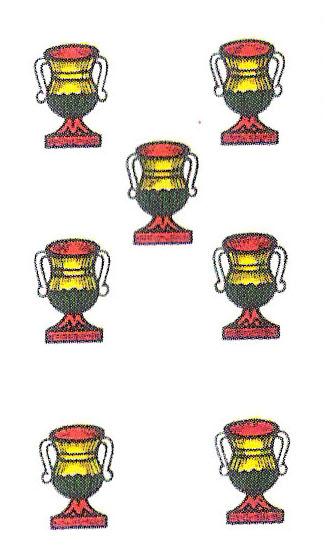
\includegraphics[width=.15\textwidth]{img/7C.jpg}
  \\[\smallskipamount]
  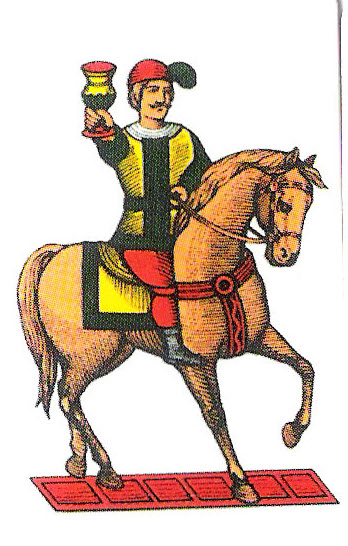
\includegraphics[width=.15\textwidth]{img/9C.jpg}\hfill
  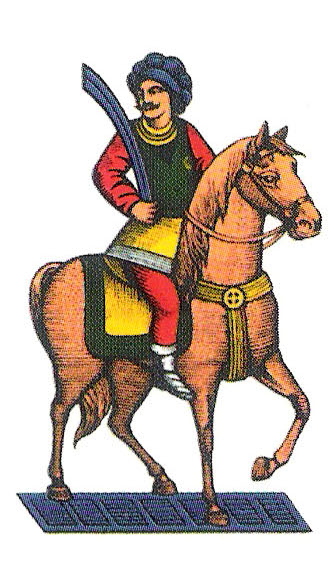
\includegraphics[width=.15\textwidth]{img/9S.jpg}
  \caption*{In order: a card with a special symbol, a basic suit card and 2 very similar cards}
\end{figure}

In this case, colour serves as an invaluable additional feature, complementing the existing shape characteristics to improve classification accuracy.
In total, we need to reliably identify 22 individual shapes:

\begin{itemize}
  \item the 8, 9 and 10 cards are counted once.
  \item the basic suits to count
  \item the 4 of Assi and other cards with special shapes, such as the 2 of Swords
  \item other cards with special symbols, such as the 5 of Swords
\end{itemize}


\begin{figure}[H]
  
\includegraphics[width=.15\textwidth]{img/5S.jpg}\hfill
  
\includegraphics[width=.15\textwidth]{img/2S.jpg}
  \caption*{On the left is a card with special symbols. On the right is a unique card shape.}
\end{figure}


\subsection*{Experiment Platform}
The following equipment and software was used to bring the project to life:
\begin{itemize}
  \item Pixel 6a with stock camera application for taking photos;
  \item Python 3.11.5
\end{itemize}


\subsection*{Pipeline}
The Neapolitan Card Recognizer (NCR) project uses a pipeline that integrates image pre-processing, dataset generation with perspective transformations, feature extraction focusing on shape and colour, and the use of machine learning for card classification. This structured approach ensures accurate recognition of Neapolitan playing cards from images, overcoming challenges such as image quality and variability through extensive pre-processing and the use of a RandomForestClassifier for card type identification.

\begin{figure}[H]
  \centering
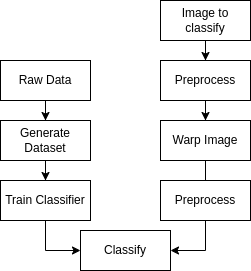
\includegraphics[width=.26\textwidth]{img/genralDescription.png}
\caption*{The pipeline used for the card capture and identification} 
\end{figure}


\subsection*{Card Detection}
The effectiveness of NCR depends largely on the robust detection of playing cards in a complex background. This section describes the comprehensive methodology used for card detection, detailing the steps from initial image acquisition to isolation of potential card regions for further processing and classification.

\begin{figure}[H]
  \centering
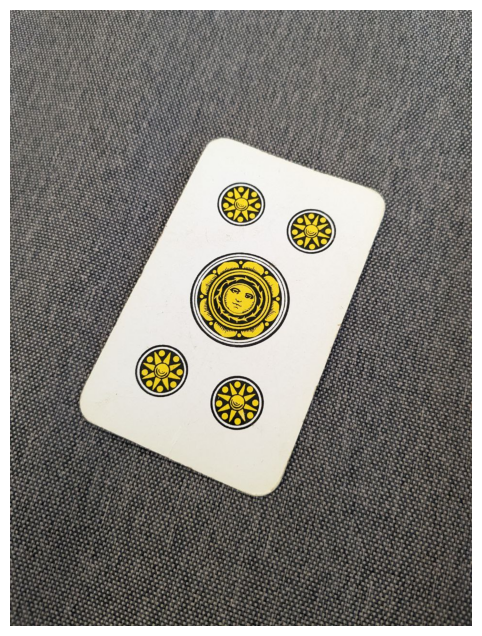
\includegraphics[width=.26\textwidth]{img/1-raw.png}
\caption*{Raw Image} 
\end{figure}

The journey begins with the acquisition of a high-resolution image, which is then subjected to a series of pre-processing steps aimed at simplifying the detection process. Given the high resolution of the images captured by the camera used, which can inadvertently highlight small imperfections on the card surface or background, an initial downsampling step is applied. This downsampling effectively reduces the image size by a factor of two, striking a balance between preserving essential detail and minimising unnecessary complexity.

We then apply a morphological operation to smooth the image morphology, creating a more uniform background and making it easier to isolate the card from the rest of the image. Specifically, a 3x3 kernel closure operation is used, which is effective in reducing noise and small imperfections on the card and background.



\begin{figure}[H]
  \centering
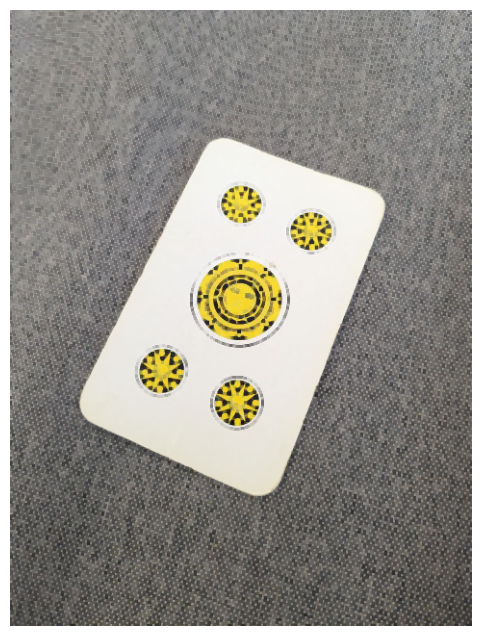
\includegraphics[width=.26\textwidth]{img/downsampled_and_morphed.png}
\caption*{Simplified image} 
\end{figure}


After pre-processing, the image undergoes a binary conversion process. This critical step transforms the image into a binary format that makes the card stand out against its background, making it easier to see its contours. A more detailed explanation of pre-processing can be found in the relevant subsection.

\begin{figure}[H]
  \centering
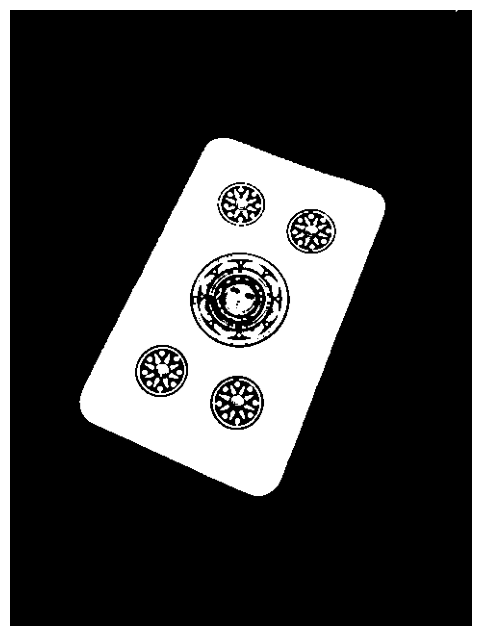
\includegraphics[width=.26\textwidth]{img/binary.png}
\caption*{Binarized Image} 
\end{figure}

To filter out insignificant contours, those too small to be cards, we order them in a decrescent manner based on the dimension of the area they occupy. The contours are then approximated using the \textbf{cv2.approxPolyDP}. The first contour with an area large enough in relation to the size of the image and with 4 corners is considered as the card to be identified.

\begin{figure}[H]
  \centering
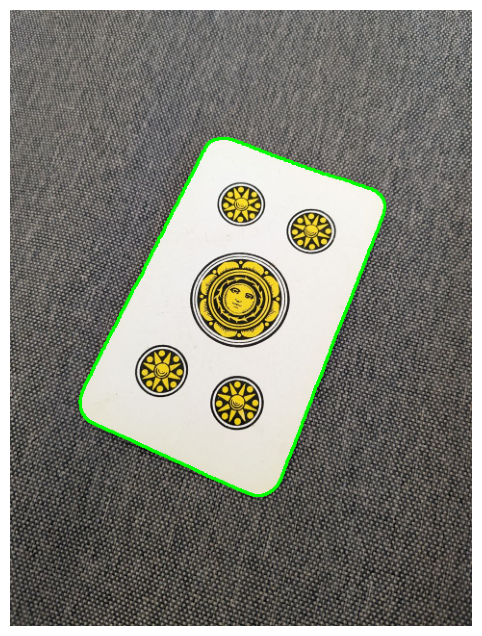
\includegraphics[width=.15\textwidth]{img/2-cardIdentified.png}\hfill
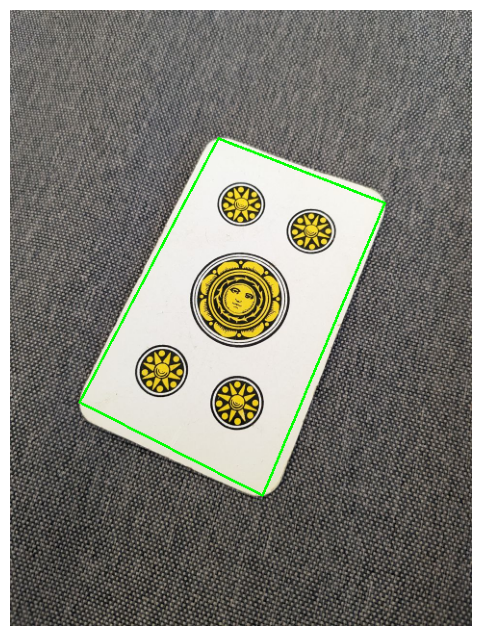
\includegraphics[width=.15\textwidth]{img/approx_card.png}\hfill
\caption*{Identified card Image and its approximated contour} 
\end{figure}

The corner points are then identified as the topLeft, topRight, bottomLeft and bottomRight corners, assuming that the card is more or less in a vertical position with respect to the frame. This is done using the fact that if we sum the coordinates of the points, the topLeft corner will have the minimum value and the bottomRight the maximum and if we differentiate the coordinates, the topRight will have the minimum value and the bottomLeft the maximum.

\begin{figure}[H]
  \centering
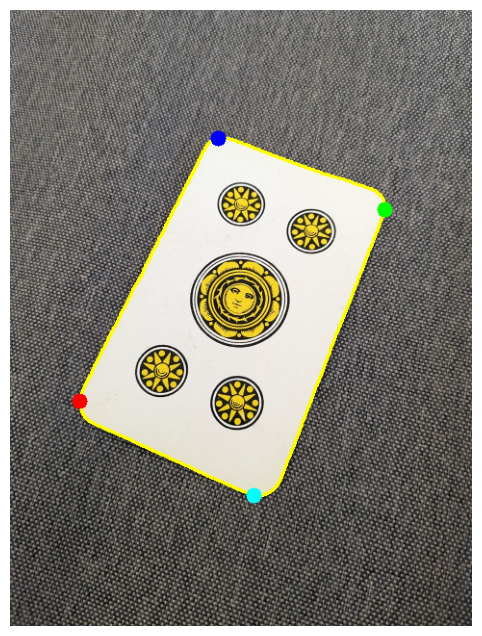
\includegraphics[width=.26\textwidth]{img/3-corner.png}
\caption*{Corners of the card} 
\end{figure}

These corners are then used to warp the perspective, defining the new image dimensions using the maximum width between the top and bottom corners and the maximum height between the left and right corners. Then the new image is generated using the \textbf{cv2.getPerspectiveTransform} to get the warp matrix and the \textbf{cv2.warpPerspective} with the new dimensions to get the final result.

\begin{figure}[H]
  \centering
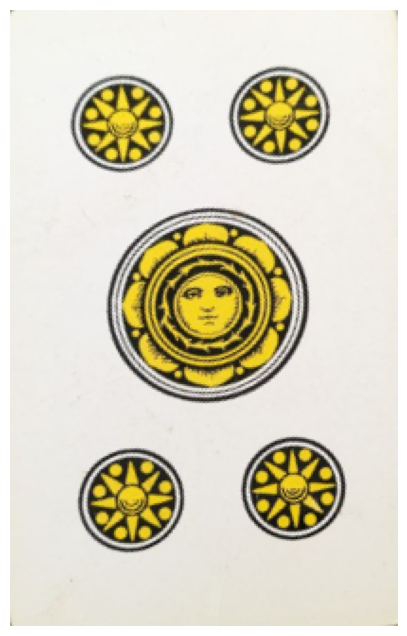
\includegraphics[width=.26\textwidth]{img/4-warped.png}
\caption*{Warped card} 
\end{figure}

\subsection*{Preprocessing}

Pre-processing serves as a critical foundation for the subsequent detection and recognition of Neapolitan cards. This stage includes several key procedures designed to improve image quality and isolate features critical for accurate classification. The comprehensive pre-processing pipeline includes white balance correction, greyscale conversion, median blurring, image inversion and contrast enhancement, and contour extraction. Each step is tailored to the specific challenges posed by the raw images and is critical to the robust performance of the NCR.
 
\begin{figure}[H]
  \centering
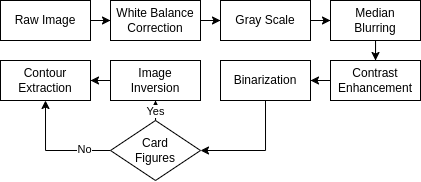
\includegraphics[width=.4\textwidth]{img/Preprocessing-Pipeline.png}
\caption*{The pipeline used for the card capture and identification} 
\end{figure}

\subsubsection*{White Balance Correction}
Given the variability of the lighting conditions under which images may be captured, and the inconsistencies introduced by the camera application's automatic white balance, a white balance correction step is applied to ensure colour consistency across different images. This step adjusts the colour temperature of the image so that the colours appear more natural and consistent, which is crucial for accurate feature extraction and classification later in the process.

The correction process involves converting the image to a floating-point representation to calculate the average value for each colour channel (blue, green and red). Scaling factors are then calculated to adjust each channel's average to match the overall average brightness, effectively neutralising colour casts caused by different lighting conditions.
\begin{figure}[H]
  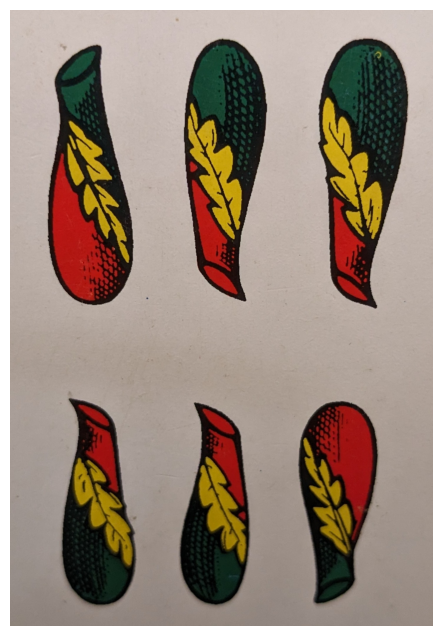
\includegraphics[width=.23\textwidth]{img/w1.png}\hfill
  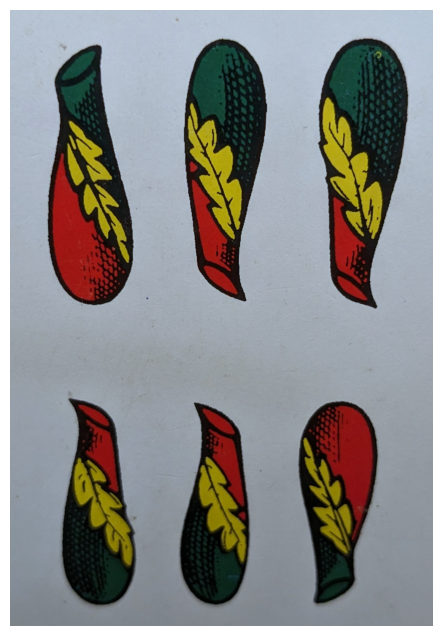
\includegraphics[width=.23\textwidth]{img/w2.png}

  \caption*{Card before and after white balance}
\end{figure}

\subsubsection*{Grayscale Conversion and Median Blurring}

To simplify contour detection and reduce computational complexity, the image is converted to greyscale using the \textbf{cv2.cvtColor} function. This conversion discards colour information and focuses on intensity variations (in 256 levels), which are essential for identifying card shapes and features.

After the greyscale conversion, a median blur is applied to the image using the \textbf{cv2.medianBlur} function with a 3x3 kernel. This type of blur is effective in reducing noise and minor imperfections such as dust specks without significantly blurring the edges of the card. It helps to clean up the image without severely affecting the contours of the image, and without the use of edge-preserving filters, which could degrade performance. This is particularly important when capturing large amounts of data.

\subsubsection*{Contrast Enhancement}
After median blurring, the image undergoes a contrast enhancement step. This is achieved by adjusting the contrast and brightness levels of the image, making the features of the card more pronounced and easier to see. This is done using the \textbf{cv2.convertScaleAbs} function. Increased contrast is particularly useful for highlighting the edges and details of cards, which are critical for accurate identification.

\subsubsection*{Binarization}
Once we have the best possible card image, we can binarise the image (convert each pixel into a 1 or 0). Considering that we are working with cards that have a fairly uniform background and high contrast, we can use a high threshold to set pixels to 1. We use the \textbf{cv2.threshold} with a threshold of 155.

\subsubsection*{Image Inversion and Contour Extraction}
For contour extraction, we need to distinguish between when we have photos of black subjects on white backgrounds (identifying card shapes on the white of the card background) and the reverse (mostly white cards on a dark background).

Since the contour extraction function \textbf{cv2.findContours} works in the second case, we need to implement a function to invert the binary values from the binarisation when identifying the figures on the card.

This process involves identifying continuous curves that delineate the boundaries of the card from the rest of the image. Contours are detected by applying edge detection algorithms to the pre-processed image, followed by retrieving outlines that represent potential card shapes.

The contours are then sorted and possibly filtered based on their occupied area to ensure that only relevant contours that are likely to represent cards or card figures are considered in subsequent processing stages. This selective approach streamlines the recognition process and focuses computational resources on the most promising candidates.
\\
\subsection*{Dataset}
The creation of a robust and diverse dataset is central to the development of any machine learning system, including the Neapolitan Card Recogniser (NCR). This section outlines the methodology used to generate a comprehensive dataset of Neapolitan cards, focusing on the techniques used to simulate a wide range of real-world conditions in which the cards might be photographed.

\subsubsection{Initial Setup and Preprocessing}
The dataset creation process begins with a collection of high quality digital scans of Neapolitan cards. These scans are manually cropped to isolate individual cards, ensuring clarity and consistency across the initial dataset. A perspective transformation is then applied to create a more robust classifier. 

\subsubsection{Perspective Transformation}
A key step in the data enhancement process is the application of perspective transformations to the card images. This process simulates the effect of taking photographs from different angles and distances, introducing realistic distortions similar to those seen in everyday use. A random perspective change is then applied.

The aim is to generate a unique perspective matrix for each image based on random parameters. The parameters for the matrix are determined using a combination of fixed seeds for repeatability and random number generation to introduce controlled randomness into the transformation process.
\begin{equation}
  \centering
  \begin{bmatrix}
    1+r & 0+r & 0+r\\
    0+r & 1+r & 0+r\\
    0 & 0 & 1+r
  \end{bmatrix}
\end{equation}
\captionof{mat}{Perspective matrix used for transformation. The value "r" is a random value between -0.02 and 0.02, different for each element of the matrix.}

To accommodate the distortion without cropping the card images, each card is first placed in the centre of a larger canvas before perspective transformation. This step ensures that the entirety of the card remains visible after the transformation, regardless of the distortion applied.

Each card image undergoes the random perspective change a predetermined number of times (in this case 24 iterations per card). This process results in a significantly expanded dataset, with each original image yielding 24 uniquely transformed variants. These variants are stored in a new dataset directory, systematically labelled to facilitate easy identification and retrieval.

\begin{figure}[H]
    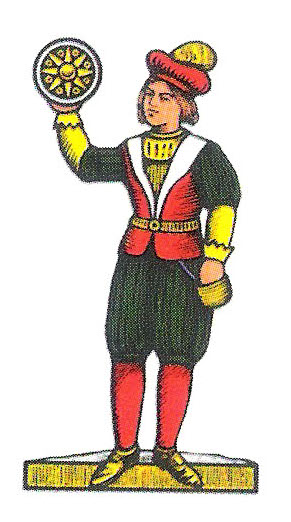
\includegraphics[width=.15\textwidth]{img/w_cards/w_card1.jpg}\hfill
    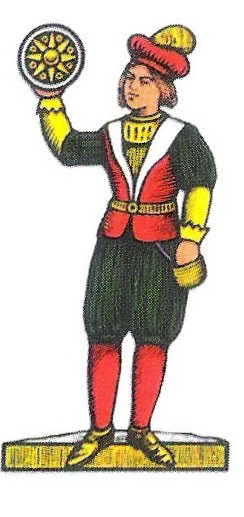
\includegraphics[width=.15\textwidth]{img/w_cards/w_card2.jpg}
    \\[\smallskipamount]
    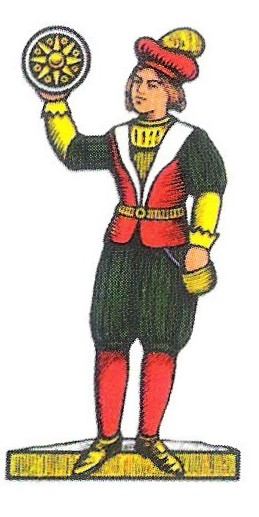
\includegraphics[width=.15\textwidth]{img/w_cards/w_card3.jpg}\hfill
    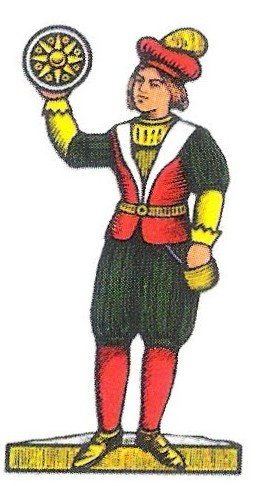
\includegraphics[width=.15\textwidth]{img/w_cards/w_card4.jpg}
    \caption*{Original card and 3 warped versions}
\end{figure}

The labels contain both the characteristics of the card (value, seed) and the iteration of the transformation, allowing precise tracking of data provenance and characteristics.

Each processed image, complete with detected contours, is saved back to the working directory to allow manual checking of the effectiveness of the generation.

\subsection*{Classification}

The classification stage is the culmination of the Neapolitan Card Recogniser (NCR) process, where the system uses machine learning algorithms to accurately identify the type of card present in an image. This section details the methodology used in the card classification process, highlighting data preparation, feature extraction, model training, evaluation and the use of the classification model to predict card types.

\subsubsection*{Data Preparation and Feature Extraction}
The classification process begins with the preparation of a dataset consisting of images of Neapolitan cards that have been subjected to perspective transformations to simulate real-world conditions. Each image in the dataset is processed to extract two main types of features: Hu moments and mean hue. The Hu moments are used to capture the shape information of the cards, while the average hue captures the colour information, both of which are crucial for distinguishing between different types of Neapolitan cards.

Hu moments: These moments are computed for the largest contour of each card, providing a seven-element feature vector describing the shape of the card. These features are scale and rotation invariant, useful not only for the part of the perspective change not corrected by the card capture step, but also for identifying the rotated shapes of the basic suits.  These moments were calculated using the function \textbf{cv2.HuMoments} applied to the moments obtained with \textbf{cv2.moments}.

\begin{figure}[H]
  \centering
  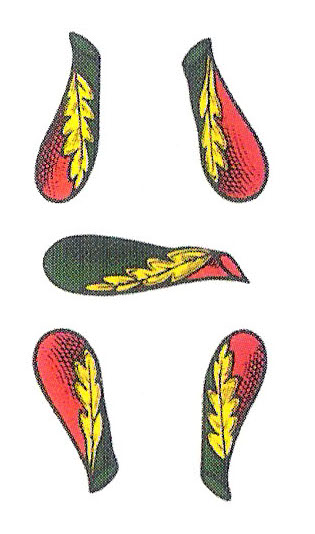
\includegraphics[width=.23\textwidth]{img/5B.jpg}

  \caption*{Card with the same basic contour repeated and rotated}
\end{figure}

Average Hue: This feature represents the average colour hue within the contour of the card, adding an extra dimension to the feature set. This value is obtained by averaging the hue value obtained in the pixels within the contour after the image has been converted to the HSV colour space.
This conversion was used to obtain a single value to consider for colour, to avoid adding too many features to classify from.

All these features are then concatenated to form a comprehensive feature vector for each card, which serves as input to the machine learning model.

\subsubsection*{Model Training}
For the classification model, a RandomForestClassifier from the scikit-learn library is chosen due to its effectiveness in handling non-linear data and its ability to model the complex relationships between the shape and colour features of the cards. The dataset is split into training and test subsets to accurately assess the performance of the model. A standard scaler is applied to the feature vectors to normalise the data and ensure that the model is not biased by the scale of the features.

The RandomForest model is trained on the normalised training data, where the label for each image indicates the type of Neapolitan card (e.g. "RO" for "Re" of "Oro"). For the cards with basic suits to be counted, the label is only the suit type: B for "Bastoni", S for "Spade", O for "Oro" and C for "Coppe". The number of estimators for the RandomForestClassifier is set to 10, providing a balance between model complexity and performance.

\subsubsection*{Evaluation and Prediction}
After training, the accuracy of the model is evaluated on the test subset of the dataset. The accuracy score and a detailed classification report provide insight into the model's performance across different card types. In addition, a confusion matrix is generated to visualise the model's predictions against the true labels, highlighting areas where the model may be confusing one card type for another. \ref{fig:c_matrix}.

\begin{figure}
  \centering
  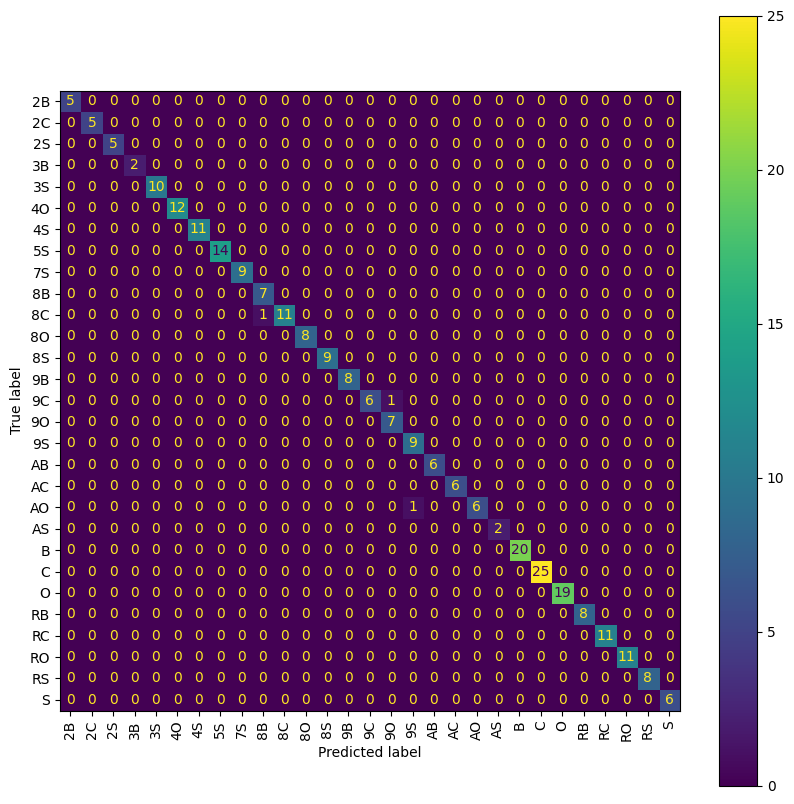
\includegraphics[scale=0.4]{img/confusionMatrix.png}
  \caption{Confusion Matrix that represent accuracy using the generated dataset. The contours to count are labeled as basic Suits [B,C,O,S]}
  \label{fig:c_matrix}
\end{figure}

For cards that fall into the category of simple shapes that can be counted (for example, the 7 of "Bastoni"), we can predict the other "smaller" contours and see if they are of the same type.

The trained RandomForest model, together with the scaler, is then stored on disk for future use in classifying new card images.

\section*{Conclusion and Future Developments}

The Neapolitan Card Recognizer project represents a study advancement in the application of machine learning and computer vision techniques to the identification and classification of traditional playing cards. Through careful pre-processing, robust dataset generation and sophisticated classification methods, the NCR demonstrates high accuracy in recognising Neapolitan cards under a variety of conditions. This system not only serves as a valuable tool that demonstrates the potential for applying similar technologies to other areas of cultural heritage and digital humanities.

\subsection*{Achievements}
The development of the NCR system has highlighted several key achievements:
\begin{itemize}
  \item The creation of a versatile pre-processing pipeline that improves image quality and isolates critical features for card recognition.
  \item The creation of a pipeline that can be easily adapted for different card games.
  \item The generation of a large and diverse dataset of card images, simulating real-world conditions through perspective transformations.
  \item The implementation of a robust classification model capable of distinguishing between different types of Neapolitan cards with high accuracy.
\end{itemize}


\subsection*{Future Developments}
While the current iteration of the NCR has proven effective, there are several avenues for future development that could improve the performance and usability of the system:

\begin{itemize}
  
  \item \textbf{Simplification of the Identification Process:} One of the potential improvements is to simplify the card identification process by reducing or eliminating the need for image distortion during identification. This could involve the development of more advanced algorithms capable of recognising cards from different angles and conditions without the need for extensive pre-processing. Such simplification could significantly speed up the recognition process and reduce computational requirements.

  \item \textbf{Expansion of the Dataset:} Expanding the dataset to include a wider range of card designs, conditions and backgrounds could further improve the robustness and accuracy of the model. Incorporating user-generated content and using crowdsourcing platforms could be a cost-effective way of enriching the dataset.

  \item \textbf{User Interface Development:} The development of a user-friendly interface for both dataset augmentation and card recognition could make the NCR more accessible to a wider audience, including researchers, game developers and enthusiasts. This could facilitate the adoption of the NCR in practical applications for use with visually impaired people.

  \item \textbf{Real-time Recognition:} Implementing real-time card recognition capabilities could open up new possibilities for interactive applications, such as augmented reality games or educational tools that provide instant feedback or information about the cards.

  \subsection*{Conclusion}   
  The Neapolitan Card Recognizer project is a testament to the power of combining traditional cultural elements with cutting-edge technology. As we look to the future, the potential for further development and application of the NCR is vast and promises not only to enhance our understanding and appreciation of Neapolitan cards, but also to pave the way for innovative applications of machine learning and computer vision in cultural preservation and beyond.
\end{itemize}
\nocite{*}
\bibliographystyle{BSO2022}
\bibliography{references}
\newpage
\onecolumn
\end{document}
